\chapter{Design of a Vortex Method for the Lamb-Oseen vortex}
\label{ch:vm-design}


This chapter introduces the fluid problem to be simulated,
and the design decisions...
\todo{Terminar introducción.}

\section{The Lamb-Oseen vortex}
\label{sec:lamb-oseen-vortex}

The Lamb-Oseen vortex is the simplest viscous vortex.
It is a two-dimensional flow with circular symmetry
whose vorticity decays over time due to viscosity.

It arises as an exact solution of the Navier-Stokes equations
for the initial condition~\(ω(r, 0) = Γ_0\,δ(x) δ(y)\)%
~\cite[\S13.1]{saffman95}.

Its analytical form is:
\begin{equation}
  \label{eq:lamb-oseen-vorticity}
  ω(r, t) = \frac{Γ_0}{4πνt} \exp(-r^2/4νt),
\end{equation}
where \(Γ_0\) is the total circulation contained in the vortex
\(ν\) is the viscosity of the fluid.
and \(r^2 = x^2 + y^2\).
The tangential velocity is given by:
\begin{equation}
  \label{eq:lamb-oseen-tangential-velocity}
  u_\theta(r, t) = \frac{Γ_0}{2πr} \bigl(1 - \exp(-r^2/4νt)\bigr),
\end{equation}
which translates into the velocity vector
\(\vec{u} = (-y, x)\cdot u_\theta(r, t)/r \).

%The Lamb-Oseen vortex evolves in free space,
%so there are no solid boundaries that need to be accounted for.
%As there are no boundaries where vorticity can be generated,
%the changes in the vorticity field during the flow evolution
%are due only to diffusion.

The Reynolds number of the vortex
is typically defined as \(\text{Re} = Γ_0/ν\).

Because of its simplicity,
the Lamb-Oseen vortex is typically used
for testing viscous fluid flow simulations.
Its known analytical form allows exact error measuring,
and since it evolves in free space,
there are no solid boundaries that need to be accounted for.

Also, it can be used in practice
as a model for simple rotational phenomena.
For example,
the wing tips of a flying airplane
generate two strong counter-rotating cylindrical air masses,
whose cross-section can be described roughly as Lamb-Oseen vortices
for analytical purposes~\cite{mcgowan71}.
These trailing vortices in the wake of large aircraft
can be hazardous to other planes encountering them in flight.

\begin{figure}
  \centering
  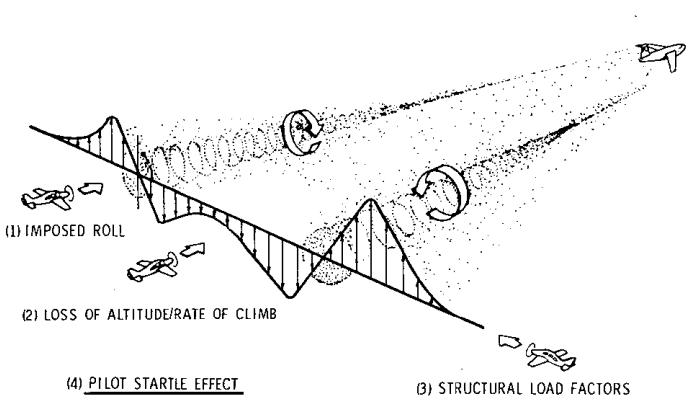
\includegraphics[scale=.5]{wingtip-vortices}
  \caption{Wing tip vortices generated by a large aircraft.}
  \label{fig:cells}
\end{figure}

\section{Discretization and initialization}
\label{sec:lamb-oseen-discretization}

The simulation for the Lamb-Oseen vortex
needs to start at a time other than zero,
because of the~\(t\) factor in the denominators
in equation~\eqref{eq:lamb-oseen-vorticity}.
\(t_0 = 4.0\) was chosen arbitrarily as a starting time.
It is the same \(t_0\) chosen by Cruz~\cite{cruz08}.

\begin{figure}
  \centering
  \includegraphics[scale=.40]{particle-init}
  \caption{Discretization of the support of the vorticity field
    into cells with a triangular distribution,
    and initial position of the particle within each cell.}
  \label{fig:cells}
\end{figure}

The initial vorticity field was first discretized into squared cells with side~\(h\)
in a so-called triangular distribution,
as shown in figure~\ref{fig:cells}.

One particle was initialized at the center of each cell.
The initial circulation of each particle
was set to an estimation of the circulation
around its containing cell,
computed as \(α_p^{(0)} = h^2\cdot ω(\x_p, t_0)\).

As the discretization is typically done on a square mesh,
the radial symmetry of the vorticity field
is broken by the particles initialized in the corners of the mesh,
introducing undesired artifacts in the integrated field.
A circulation threshold \(α^\text{max}\)
was imposed on the particle list in order to retain the symmetry.

%\fbox{\textbf{To do:} insert plot showing artifacts.}

For the later stages of the algorithm,
the particle core size was set to \(ε = 2h\).
This choice was taken from an example in~\cite[\S2.4]{cottet00},
and it ensures that particles overlap,
which is a necessary condition for convergence.
%\fbox{\textbf{To do:} check whether this is actually true, and cite a reference.}
The core size is kept constant throughout the simulation,
as the flow is incompressible.

Particle initialization is a one-time \(O(N)\) operation,
so it does not affect overall performance significantly.
It was implemented as a standalone serial program
that outputs the list of particles in plain text format.

\section{Velocity evaluation}
\label{sec:velocity-evaluation}

For a given distribution of circulation-carrying particles,
the velocity at any location can be computed
by evaluating the Biot-Savart law:
\begin{equation}
  \label{eq:biot-savart-law-velocity-evaluation}
  \vel^h(\x) = \sum_p α_p \K_ε(\x - \x_p).
\end{equation}

As this \(N\)-term sum needs to be computed
at each of the \(N\) particle locations,
velocity evaluation is an~\(O(N^2)\) operation.
This is an instance of the~\(N\)-body problem,
and is typically the most expensive stage
of a Vortex Method.

Even though there are approximate algorithms better than~\(O(N^2)\)
for evaluating the sum, as mentioned in section~\ref{ssec:vel-eval},
for this work the brute force all-pairs algorithm will be used~\cite{gems3}.
Since the \(N\)-body problem arises
in several scientific and engineering applications,
the efficient implementation of the all-pairs method in parallel architectures
has been widely studied.

\section{Trajectory integration}
\label{sec:trajectory-integration}

Once the velocity of each particle is evaluated,
their positions have to be updated
by performing one integration step
of the Lagrangian convection equation~\eqref{eq:vortex-blob-convection}.

In~\cite[\S2.2]{cottet00},
it is mentioned that velocity should be integrating
using schemes that are at least second order.
However, for this work a first-order Euler integrator will be used,
as the main goal is to assess performance.

Higher-order integration methods
evaluate particle velocities several times per time step
and need larger memory allocations.
For instance,
a fourth-order Runge--Kutta scheme
requires four velocity evaluations per particle
and four additional arrays of size~\(N\)
for storing the intermediate results.
Besides these,
there are no other algorithmic differences.

The Euler time-stepping scheme is:
\begin{equation}
  \label{eq:euler-time-stepping}
  \x_p^{(n + 1)} = \x_p^{(n)} + \vec u_p^{(n)}\cdot δt,
\end{equation}
where \(\vec u_p^{(n)}\) is the velocity of the particle
at time \(t = t_0 + n\cdot δt\)
evaluated through equation~%
\eqref{eq:biot-savart-law-velocity-evaluation}.

\section{Vorticity derivative evaluation}
\label{sec:vorticity-derivative-evaluation}

For solving the Lagrangian diffusion equation~\eqref{eq:vortex-blob-convection},
the Particle Strength Exchange scheme will be used.

PSE models diffusion as the exchange of circulation among nearby particles.
It is based on the integral approximation of the Laplacian:
\begin{equation}
  \label{eq:integral-laplacian}
  Δ_ε ω(\x) = ε^{-2} \int [ω(\x') - ω(\x)]\cdot η_ε(\x' - \x)\,d\x',
\end{equation}
where \(η_ε(\x) = ε^{-2} η(\x/ε)\) is a scaled approximation of the heat kernel.

The numerical quadrature of the integral
yields its discrete form for each particle:
\begin{equation}
  \label{eq:pse}
  Δ_ε ω_p = ε^{-2} \sum_q v_q [ω_q^h - ω_p^h]\cdot η_ε(\x_q - \x_p),
\end{equation}
where \(v_q\) is the volume of particle~\(q\).
All particles represent a initial cell of volume \(v_p = h^2\),
which would not change when moving along the stream
because of the incompressibility of the flow,
and therefore \(v_p = v_q\) for all \(p\) and \(q\).
Since circulation is related to vorticity by \(α_p = v_p ω_p\),
the PSE equation can be expressed in terms of circulation as:
\begin{equation}
  \label{eq:pse-circ}
  Δ_ε α_p = ε^{-2} \sum_q [α_q^h - α_p^h]\cdot η_ε(\x_q - \x_p).
\end{equation}

The diffusion equation~\eqref{eq:vortex-blob-diffusion} then becomes:
\begin{equation}
  \label{eq:pse-circ}
  \dot{α}_p = νε^{-2} \sum_q [α_q^h - α_p^h]\cdot η_ε(\x_q - \x_p).
\end{equation}

Just like for the convection stage,
equation~\eqref{eq:pse-circ}
yields a \(N\)-body problem.
Once again,
the all-pairs method will be used
for its evaluation.

It must be noted, though, that
because of the short-range nature
of the Laplacian operator,
most of the interactions between pairs of particles
will be practically zero.
There are methods that avoid these computations
by tracking the neighbors of each particle,
but this requires frequent remeshing of the particles
onto regular locations as the flow evolves.
The implementation of these methods
(like Verlet lists and cell lists)
on the GPU will be left as future work.

\section{Vorticity integration}
\label{sec:vorticity-integration}

As it is the case for the convection equation,
the diffusion equation has to be integrated
once the derivative is evaluated.
For this stage,
an Euler time-stepping scheme will be used as well.

A natural approach for integrating both the convection and the diffusion equations
is to do it in turns, taking first into account only the convective part of the flow,
and then making the diffusion operator act on the new particle locations.
This is known as \emph{viscous splitting},
and is the basis of several diffusion models.
Viscous splitting limits the order of accuracy of the integration scheme
(its basic two-step form is only second-order accurate
at each time step~\cite[\S2.1.1]{barba04}).

The Particle Strength Exchange method
does not require to be formulated
in a viscous splitting frame.
The velocity and the derivative of the vorticity
can be evaluated at the same time step,
and both convection and diffusion equations
can also be integrated simultaneously.

The Euler time-stepping scheme for the diffusion is:
\begin{equation}
  \label{eq:euler-diffusion}
  α_p^{(n + 1)} = α_p^{(n)} + \dot{α}_p^{(n)}\cdot δt,
\end{equation}
where~\(\dot{α}_p\) is the derivative of the circulation
evaluated by the Particle Strength Exchange method
as in equation~\eqref{eq:pse-circ}.

